%%%%%%%%%%%%%%%%%%%%%%%%%%%%%%%%%%%%%%%%%%%%%%%%%%%%%%%%%%%%%%%%%%
%%%%%%%% ICML 2014 EXAMPLE LATEX SUBMISSION FILE %%%%%%%%%%%%%%%%%
%%%%%%%%%%%%%%%%%%%%%%%%%%%%%%%%%%%%%%%%%%%%%%%%%%%%%%%%%%%%%%%%%%

% Use the following line _only_ if you're still using LaTeX 2.09.
%\documentstyle[icml2014,epsf,natbib]{article}
% If you rely on Latex2e packages, like most moden people use this:
\documentclass{article}

% use Times
\usepackage{times}
% For figures
\usepackage{graphicx} % more modern
\usepackage{booktabs}
%\usepackage{epsfig} % less modern
\usepackage{subfigure}

% For citations
\usepackage{natbib}

% For algorithms
\usepackage{algorithm}
\usepackage{algorithmic}

% As of 2011, we use the hyperref package to produce hyperlinks in the
% resulting PDF.  If this breaks your system, please commend out the
% following usepackage line and replace \usepackage{icml2014} with
% \usepackage[nohyperref]{icml2014} above.
\usepackage{hyperref}

% Packages hyperref and algorithmic misbehave sometimes.  We can fix
% this with the following command.
\newcommand{\theHalgorithm}{\arabic{algorithm}}

% Employ the following version of the ``usepackage'' statement for
% submitting the draft version of the paper for review.  This will set
% the note in the first column to ``Under review.  Do not distribute.''
\usepackage{icml2014}


% The \icmltitle you define below is probably too long as a header.
% Therefore, a short form for the running title is supplied here:
\icmltitlerunning{O'Meara, Stephani, Hand}

\begin{document}

\twocolumn[
\icmltitle{Project Report for CIS 419/519\\Stock Recommendations using Machine Learning}

% It is OKAY to include author information, even for blind
% submissions: the style file will automatically remove it for you
% unless you've provided the [accepted] option to the icml2014
% package.
\icmlauthor{Michael O'Meara}{momeara@seas.upenn.edu}
\icmlauthor{Timmy Stephani}{stephan6@seas.upenn.edu}
\icmlauthor{Dave Hand}{handd@seas.upenn.edu}

% You may provide any keywords that you
% find helpful for describing your paper; these are used to populate
% the "keywords" metadata in the PDF but will not be shown in the document
\icmlkeywords{machine learning, stocks, comparison, naive bayes, svm, neural networks}

\vskip 0.3in
]

\begin{abstract}
In this report, we present a simplified stock recommendation system. This system is based on patterns found from the price history of a list of equities. In developing the system, various machine learning techniques were tested to try to predict which stocks should be bought or sold to maximize the percent return going forward. We chose to use naive bayes, neural networks, and a support vector machines with a gaussian kernel as our main machine learning techniques. We trained each model on past data through a backtesting module and then presented each model with new data in order to make predictions. In addition, we utilized our module to test several different combinations of features and compared the accuracy, precision, recall, and percent return of various models.
\end{abstract}

\section{Introduction}
Many financial institutions and investors are wary of trading in the stock market since the financial collapse in 2008.  Almost all financial institutions have turned to machine learning or other algorithmic techniques in order to reduce the risk in trading. These techniques are used both in high-frequency trading and longer-term trades based on a buy and hold strategy. Our system is targeted as a longer-term trade recommendation system, avoiding the real-time constraints of high-frequency algorithms. We attempt to solve a small subset of this larger financial landscape, making good short-term predictions for buying or selling stocks that the average investor might be able to utilize.

The principle of our trading strategy is based on the idea that price movements in a stock form technical patterns that represent the sentiment of a particular equity over time. These patterns can help predict the future price movement of a stock, which if known, can improve the overall return for an investor.  In order to simplify our recommendation model we have limited our selection to the stocks in the Dow 30 and only look at closing price for the stocks in our list as the basis of our predictions.

\subsection{Model assumptions}
In our implementation, we make several assumptions to simplify the constraints. We believe that while these assumptions necessarily make the algorithms we develop less applicable to the real world, they still remain close to from reality. We believe that some of our models could potentially be used by individuals in the real world at some rate of success, but at their own risk. We first assume that the trader has stock in whichever stocks our model was trained on. This allows us to to predict whether to buy, sell, or hold regardless of whether or not the individual actually owns any stock at that current point in time. Our model can be viewed as the global prediction of whether to buy, sell, or hold on a certain day and is not related or tied to any specific trader portfolio.

An additional assumption will be that the closing price reflects the sentiment of that day's price action enough to be considered the price for the entire day. This has the added benefit of avoiding intraday fluctuations in the stock market. We will also ignore all transaction fees and taxes associated with trading on the stock market and simply use a flat fee of 0.5\%.

\subsection{Definition}
Our models were compared on several different characteristics, including many baseline machine learning metrics. In addition, we calculated the percent return that our model would have produced if it was followed every day of the test. This was calculated so that we could compare it to the actual return of the stock over the same period of time. That way, we could empirically see that our model was outperforming the average case. The formula for calculating the percent return is:

$$
Percent Return = \frac{(V_{now} - V_{beginning})}{V_{beginning}}
$$

\section{Methodology}

\subsection{Source of data}
The dataset used was downloaded from Wharton Research Data Services (WRDS). The stocks used are the stocks that comprise the Dow30. The Dow30 is an index of stocks developed as a way of tracking U.S. market performance. It is comprised of the current top thirty blue-chip U.S. stocks. For each stock, we pulled several features, including closing price, high, low, and volume. Our research into the field suggested that these features would be the best for prediction. We pulled stock data from January 1, 1983 to December 31, 2013 to give us a window of 30 years. WRDS does not currently store the data we were utilizing for 2014.

The closing price is the price at the end of a particular time period. The daily closing price is the price at the end of a day. The high and low are the spread between what the buyer must pay for a stock (high) and what the seller would receive for a stock (low). The volume is the number of shares that were traded on a given day for a stock.

The features we used could be pulled in different time frames. For instance, we could pull yearly, monthly, or daily records for closing price. However, our research into the field suggested that a daily time frame would be both the best to predict on and the most desired model as well. Most successful papers trained daily models on past flucutations. In addition, predicting on monthly or yearly changes in the stock market is not as applicable to the individuals who would want to use this.

\subsection{Trading strategy}
The strategy each of our models is designed for is determining exactly when it is time to buy and sell stocks as well as when to simply hold steady. Therefore, we have a choice of three classes to assign to each time frame in our model. Our model assigns its choice based on the threshold of the transaction fee of 0.5\% we assigned above. If the model is expecting a change of more than 0.5\% either way, the model will choose to buy or sell accordingly. Otherwise, it will predict to hold. This decision is because it does not make sense to make a trade when the percentage difference is less than the fee to make the transaction. We then compare the model's choice with the actual best decision, which is calculated with the actual percent change in the same manner, in order to determine if the model's choice was correct. All predictions, including hold, are counted as successful "trades" if they match the actual best decision. The number of successful trades divided by the number of possible successful trades is how we obtain our accuracy. Calculations for precision and recall are related to the number of successful trades as well.

\subsection{Backtesting}

We have written a backtesting module to look at different time frames and feature sets in our historical trades data. The backtesting module also allows us to choose where our time frame begins and ends, i.e. if we only wanted to use 2013 data for our training and testing. After researching how it is done in the real world, we have also implemented pattern recognition in our backtesting code to confirm that there are trends we could exploit.

After some runs with different inputs with the backtesting module, we began to deduce that the best time frame for training and testing was daily data, not monthly or yearly. The monthly or yearly data simply produced very bland patterns when compared to the patterns produced by daily data. BETTER EXPLANATION. We decided we would utilize daily data when training our models in order to achieve the best, and more importantly, most realistic data.

Section 3.5 shows some example patterns that our system found with the current pattern in cyan.   The other lines are past patterns that our system found that are potential matches and the dots to the right represent outcomes for each past pattern.  The rightmost dots are the actual outcome and average of the past patterns.

\subsection{Machine learning framework}

At this point, we've also set up another framework that allows us to easily evaluate different classifiers, different amounts of data, and different features easily. This will help us decide which classifiers, features, and data to use to train each respective machine learning model for best results.

We've also reviewed numerous published papers to understand what existing work has been done, both successful and unsuccessful, which will ultimately aid in narrowing the scope on our final evaluation and help us determine best train and test practices.

\subsection{Training and Analysis Overview}
We trained and analyzed the performance of each of the following models: naive bayes, SVM with gaussian kernel, and neural network. Each model was trained with the help of the backtesting module. MORE INFO HERE OR IS ABOVE ENOUGH? Each of the models were trained on the same stocks, time frame, and features.

We define a trade as a prediction. Every day a prediction must be made, whether to buy, sell, or hold the stock. Whether or not this prediction is the correct prediction is the heart of our model. We are attempting to predict the correct trade as often as possible based on previous data in the model.

Our models utilize the percent change of the various features they are given in order to determine whether to buy, sell, or hold. SHOULD WE SAY THE THRESHOLD AND STUFF, REALLY DUMBS IT DOWN. BOTH HERE AND IN TRADING STRATEGY. SHOULD SAY WE USE THE PERCENTAGE CHANGE TO DETERMINE WHAT THE BEST DECISION WAS. SHOW FIGURES HERE.

We used several metrics to evaluate our model, including accuracy, precision, and recall. In addition to those base metrics, we also calculated the percent return as defined above in order to better determine the financial success of our model. For example, our model could predict very well, but perhaps only gain a little on each correct prediction and lose a lot on each incorrect prediction. Therefore, percent return provides a way to verify that our correct predictions are more than just correct, they need to also be profitable. We can determine if our percent return is successful by comparing it with the stock's average actual percent return over the same period. If we outperform the actual average percent return, we consider our model to be successful.

For each model, our main focus was on model accuracy and maximizing the percent return. We wanted to produce a model that could not only beat the average return, but produce the best return possible given its training and input data.

FOCUSED ON MAXIMIZING PERCENT RETURN
several features including the price and volume history of a list of equities
could talk about data normalization

either here or before this we need to talk about how all models had the best success with a daily time frame and a single feature, but mention we tried combinations of them. Talk about how for the analysis in this paper, we used the last 100 days of 2013.

talk about how we found that all 3 classifiers did the best with just closing price - maybe because some features are not independent in finance, didn't help us to have additional features, only contributed to overfitting

talk about the most important models either here or above

talk about being trained on ony one stock at a time, model doesn't handle multiple stocks well

future work - try and predict the percent change so traders know if it's worth the risk as opposed to predicting what to do

is it worse than random guessing even though we have three options - maybe we could talk about how our predictions aren't statistically significant

\section{Model Analysis}

\subsection{Naive Bayes}
The first machine learning classifier we analyzed was naive bayes. Through research into past papers on the topic, it appeared many people had mixed results when trying to use naive bayes to predict. We did not expect naive bayes to perform well, but we did expect it to perform better than random guessing as it was still being trained on actual data. We tested multiple time frames with our naive bayes implementation, including yearly, monthly, and daily data. We also tested many different combinations of features in order to see if different feature sets changed how the model performed.

Unfortunately, we were never able to achieve statistically significant results with our naive bayes implementation. We averaged right around 51\% accuracy and a 16\% return for the model, which more or less equates to random guessing. The percent return also hovered right around the average return for the Dow30 over the same time frame, so we had not achieved a better than average return either.

NEED TO TALK ANYMORE ABOUT THIS

For comparative purposes to the other more successful models analyzed below, here is the naive bayes model's performance on each of the thirty stocks we analyzed.

NAIVE BAYES TABLE

ENDING?

\subsection{SVM (gaussian)}
The second machine learning classifier we analyzed was a support vector machine with a gaussian kernel. Research into using support vector machines in the past had given us insight into how successful these models could be. We expected the svm to perform very well on the data and to provide us with a better return on the Dow30 than the average. After tuning the parameters with a lengthy grid search, we found that our optimal svm had very respectable predictive power.

On average over the thirty stocks, our svm model predicted the correct trade with an accuracy of 67.97\%. We also averaged a 34.93\% return over the thirty stocks, meaning that we more than doubled the average percent return over the same time frame. It is important o note that the predictions and percent return are based on a simplified model, without factoring in transaction costs. However, these returns are still much higher than average, and could be useful for many traders on the stock market.

NEED TO TALK MORE ABOUT THIS? WHY WAS SVM SUCCESSFUL? WHY DID WE THINK THE SVM WOULD BE SUCCESSFUL?

The results for each of the Dow30 stocks are displayed below.

\begin{table}[h]
  \begin{tabular}{@{}lllllll@{}}
    \toprule
    Ticker & Accuracy & Precision & Recall & \% Return & \\ \midrule
    MCD & 90 & 81 & 90 & 48.99 & \\
    XOM & 85 & 72.25 & 85 & 48.27 & \\
    KO & 82 & 67.24 & 82 & 42.51 & \\
    GE & 74 & 54.76 & 74 & 41.33 & \\
    MMM & 79 & 62.41 & 79 & 40.95 & \\
    PFE & 76 & 57.76 & 76 & 40.48 & \\
    IBM & 72 & 51.84 & 72 & 38.91 & \\
    VZ & 62 & 38.44 & 62 & 38.44 & \\
    JNJ & 78 & 60.84 & 78 & 38.08 & \\
    MRK & 84 & 70.56 & 84 & 37.72 & \\
    PG & 73 & 53.29 & 73 & 37.48 & \\
    UNH & 64 & 40.96 & 64 & 36.74 & \\
    WMT & 83 & 68.89 & 83 & 36.73 & \\
    AXP & 64 & 40.96 & 64 & 36.05 & \\
    T & 68 & 46.24 & 68 & 34.65 & \\
    CAT & 70 & 49 & 70 & 34.6 & \\
    V & 59 & 34.81 & 59 & 33.8 & \\
    CSCO & 69 & 47.61 & 69 & 33.57 & \\
    INTC & 66 & 43.56 & 66 & 32.81 & \\
    JPM & 65 & 42.25 & 65 & 32.71 & \\
    DD & 70 & 49 & 70 & 32.51 & \\
    BA & 53 & 28.09 & 53 & 32.16 & \\
    G & 72 & 51.84 & 72 & 31.3 & \\
    HD & 67 & 44.9 & 67 & 30.08 & \\
    MSFT & 61 & 37.21 & 61 & 29.65 & \\
    NKE & 68 & 46.24 & 68 & 29.22 & \\
    GS & 56 & 31.36 & 56 & 28.28 & \\
    UTX & 63 & 39.69 & 63 & 28.25 & \\
    DIS & 59 & 34.81 & 59 & 27.64 & \\
    C & 53 & 28.09 & 53 & 26.99 & \\
    TRV & 48 & 23.04 & 48 & 13.71 & \\ \bottomrule
    Average & 68.80 & 48.35 & 68.80 & 34.66 & \\
  \end{tabular}
  \caption{SVM Results for the Dow30}
  \label{my-label}
\end{table}

The svm accuracy does fluctuate quite a bit between some of the stocks, having higher predictive power for some (MRK, MCD) and less for others (TRV, V). Through some deeper digging, this appears to be the result of the svm performing better on more stable stocks (segements such as drugs, food, and retail) when compared to more volatile stocks (segements such as insurance and finance). This was an interesting corollary we saw to our main findings.

IS COROLLARY THE CORRECT WORD?

\subsection{Neural network}
The final machine learning classifier we analyzed was a neural network. There was some papers we found analyzing neural network performance, but we mainly decided to try it as many quantitative finance teams in industry utilize neural networks in order to make predictions on current market trends. Faced with this knowledge, we expected the neural netowrk to perform well and outperform the Dow30 average percent return.

TALK ABOUT BACKPROP THING WE FOUND AND RANDOM RULE MICHAEL WENT WITH

On average over the thirty stocks, our neural network performed the best of the three models we analyzed. Our neural network had an average trade prediction accuracy of 68.81\% and an average 34.66\% return. We more than doubled the average return of the Dow30 over the same time period. The results here are slightly more optimistic than they should be, as our model was trained and predicted on a reduced model with a fixed transaction cost. However, the model still performs very well and would definitely prove very helpful for traders looking for an edge.

WE SHOULD SAY SVM DID BETTER BECAUSE IT HAD A SLIGHTY HIGHER PERCENT RETURN, BUT THE DIFFERENCE BETWEEN THE TWO WAS NOT THAT IMPORTANT OR SIGNIFICANT

NEED TO TALK MORE ABOUT THIS? WHY WAS NN SUCCESSFUL? WHY DID WE THINK THE NN WOULD BE SUCCESSFUL?

NN 100 epochs, ADDITIONAL DON'T HELP TOO MUCH, MUST ALREADY BE CONVERGING

The results for the neural network on all thirty stocks are printed below.

\begin{table}[h]
  \begin{tabular}{@{}lllllll@{}}
    \toprule
    Ticker & Accuracy & Precision & Recall & \% Return & \\ \midrule
    MCD & 90 & 81 & 90 & 48.99 & \\
    MMM & 79 & 62.41 & 79 & 48.95 & \\
    XOM & 85 & 72.25 & 85 & 48.27 & \\
    KO & 82 & 67.24 & 82 & 42.5 & \\
    GE & 74 & 54.76 & 74 & 41.33 & \\
    PFE & 76 & 57.76 & 76 & 40.48 & \\
    IBM & 72 & 51.84 & 72 & 38.91 & \\
    VZ & 62 & 38.44 & 62 & 38.44 & \\
    JNJ & 78 & 60.84 & 78 & 38.09 & \\
    MRK & 84 & 70.56 & 84 & 37.72 & \\
    PG & 73 & 53.29 & 73 & 37.48 & \\
    UNH & 64 & 40.96 & 64 & 36.74 & \\
    WMT & 83 & 68.89 & 83 & 36.72 & \\
    AXP & 64 & 40.96 & 64 & 36.05 & \\
    INTC & 66 & 62.46 & 66 & 35.86 & \\
    CAT & 69 & 48.79 & 69 & 34.44 & \\
    T & 67 & 46.02 & 67 & 34.18 & \\
    JPM & 65 & 42.68 & 65 & 32.71 & \\
    DD & 70 & 49 & 70 & 32.51 & \\
    V & 49 & 36.88 & 49 & 31.8 & \\
    CSCO & 63 & 49.25 & 63 & 31.48 & \\
    G & 72 & 51.48 & 72 & 31.3 & \\
    BA & 52 & 28.12 & 52 & 31.15 & \\
    MSFT & 61 & 37.21 & 61 & 29.65 & \\
    NKE & 68 & 46.24 & 68 & 29.22 & \\
    HD & 66 & 44.67 & 66 & 29.06 & \\
    GS & 54 & 43.15 & 54 & 28.47 & \\
    UTX & 63 & 39.69 & 63 & 28.25 & \\
    DIS & 58 & 34.57 & 58 & 27.46 & \\
    C & 52 & 27.84 & 52 & 26.26 & \\
    TRV & 46 & 45.12 & 46 & 18.4 & \\ \bottomrule
    Average & 67.96 & 50.14 & 67.96 & 34.93 & \\
  \end{tabular}
  \caption{Neural Net Results for the Dow30}
  \label{my-label}
\end{table}

MAYBE COMBINE OBSERVATIONS INTO OWN SUBSECTION
The neural network prediction accuracy fluctuates quite a bit on for differing stocks. The model, like the svm, had higher predictive accuracy for more stable stocks and performed worse (sometimes even worse than random guessing) for more volatile stocks.

\subsection{Overall comparison}
We had a large amount of success with two of the three models we trained, which is exactly what we expected to see. We did not predict that our successful models would perform as well as they did. Both the svm and neural network had a high percent return and accuracy. The svm performed slightly better in terms of percent return, while the neural network had a slightly higher accuracy. Both outperformed the Dow30 average percent return, meaning we can empirically state that our implementations are successful and would be useful for traders looking for an edge.

MAYBE PUT OBSERVATIONS FROM INDIVIDUAL SECTIONS HERE.

For a quick summary, here is the average performance of each of the three models over the thirty stocks.

SUMMARY TABLE

\subsection{Future Work}

Next, we plan to evaluate additional classifiers, including a neural network and naive bayes, with similar baseline variables for data and features.

As a stretch goal, we are also still trying to find additional sources of data to incorporate additional economic features into our dataset.

\subsection{Figures}

\begin{figure}[h!]
\begin{center}
        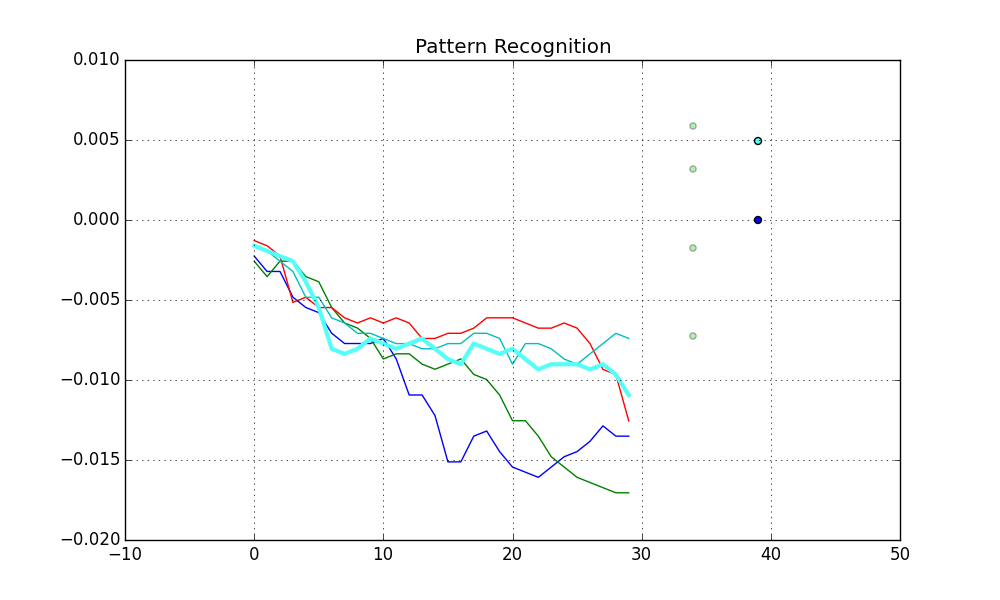
\includegraphics[scale=0.3]{figure_2}
        \caption{Examples of downward trend reversals}
\end{center}
\end{figure}

\begin{figure}[h!]
\begin{center}
        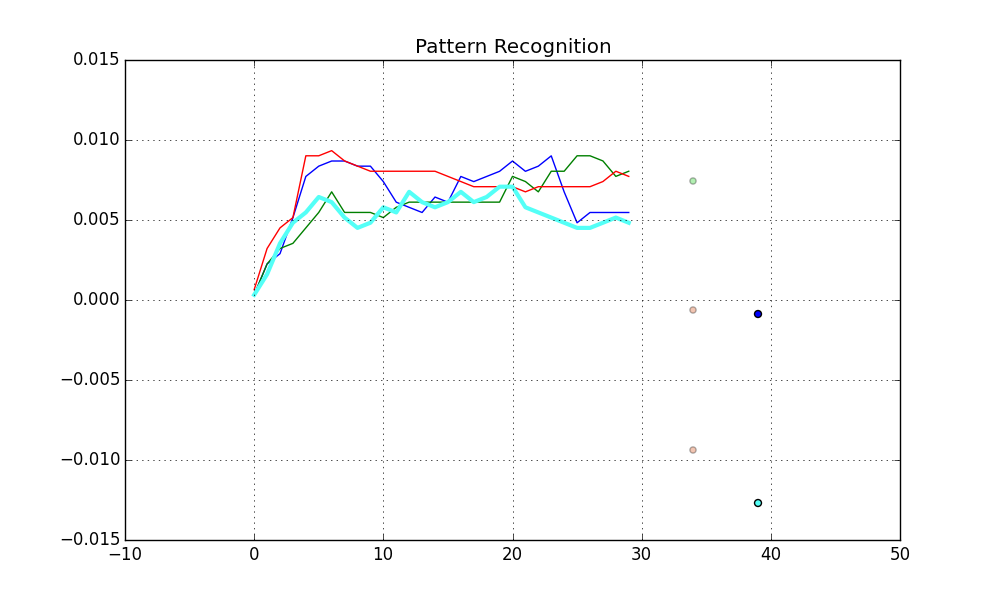
\includegraphics[scale=0.3]{figure_3}
        \caption{Examples of upward trend reversal}
\end{center}
\end{figure}

%You may want to include figures in the paper to help readers visualize
%your approach and your results. Such artwork should be centered,
%legible, and separated from the text. Lines should be dark and at
%least 0.5~points thick for purposes of reproduction, and text should
%not appear on a gray background.
%
%Label all distinct components of each figure. If the figure takes the
%form of a graph, then give a name for each axis and include a legend
%that briefly describes each curve. Do not include a title inside the
%figure; instead, be sure to include a caption describing your figure.
%
%You may float figures to the top or
%bottom of a column, and you may set wide figures across both columns
%(use the environment {\tt figure*} in \LaTeX), but always place
%two-column figures at the top or bottom of the page.
%
%\subsection{Algorithms}
%
%If you are using \LaTeX, please use the ``algorithm'' and ``algorithmic''
%environments to format pseudocode. These require
%the corresponding stylefiles, algorithm.sty and
%algorithmic.sty, which are supplied with this package.
%Algorithm~\ref{alg:example} shows an example.
%
%\begin{algorithm}[tb]
%   \caption{Bubble Sort}
%   \label{alg:example}
%\begin{algorithmic}
%   \STATE {\bfseries Input:} data $x_i$, size $m$
%   \REPEAT
%   \STATE Initialize $noChange = true$.
%   \FOR{$i=1$ {\bfseries to} $m-1$}
%   \IF{$x_i > x_{i+1}$}
%   \STATE Swap $x_i$ and $x_{i+1}$
%   \STATE $noChange = false$
%   \ENDIF
%   \ENDFOR
%   \UNTIL{$noChange$ is $true$}
%\end{algorithmic}
%\end{algorithm}
%
%\subsection{Tables}
%
%You may also want to include tables that summarize material. Like
%figures, these should be centered, legible, and numbered consecutively.
%However, place the title {\it above\/} the table, as in
%Table~\ref{sample-table}.
% Note use of \abovespace and \belowspace to get reasonable spacing
% above and below tabular lines.
%
%\begin{table}[h]
%\caption{Classification accuracies for naive Bayes and flexible
%Bayes on various data sets.}
%\label{sample-table}
%\vskip 0.15in
%\begin{center}
%\begin{small}
%\begin{sc}
%\begin{tabular}{lcccr}
%\hline
%\abovespace\belowspace
%Data set & Naive & Flexible & Better? \\
%\hline
%\abovespace
%Breast    & 95.9$\pm$ 0.2& 96.7$\pm$ 0.2& $\surd$ \\
%Cleveland & 83.3$\pm$ 0.6& 80.0$\pm$ 0.6& $\times$\\
%Glass2    & 61.9$\pm$ 1.4& 83.8$\pm$ 0.7& $\surd$ \\
%Credit    & 74.8$\pm$ 0.5& 78.3$\pm$ 0.6&         \\
%Horse     & 73.3$\pm$ 0.9& 69.7$\pm$ 1.0& $\times$\\
%Meta      & 67.1$\pm$ 0.6& 76.5$\pm$ 0.5& $\surd$ \\
%Pima      & 75.1$\pm$ 0.6& 73.9$\pm$ 0.5&         \\
%\belowspace
%Vehicle   & 44.9$\pm$ 0.6& 61.5$\pm$ 0.4& $\surd$ \\
%\hline
%\end{tabular}
%\end{sc}
%\end{small}
%\end{center}
%\vskip -0.1in
%\end{table}
%
%Tables contain textual material that can be typeset, as contrasted
%with figures, which contain graphical material that must be drawn.
%Specify the contents of each row and column in the table's topmost
%row. Again, you may float tables to a column's top or bottom, and set
%wide tables across both columns, but place two-column tables at the
%top or bottom of the page.

%Please use APA reference format regardless of your formatter
%or word processor. If you rely on the \LaTeX\/ bibliographic
%facility, use {\tt natbib.sty} and {\tt icml2014.bst}
%included in the style-file package to obtain this format.
%
%Citations within the text should include the authors' last names and
%year. If the authors' names are included in the sentence, place only
%the year in parentheses, for example when referencing Arthur Samuel's
%pioneering work \yrcite{Samuel59}. Otherwise place the entire
%reference in parentheses with the authors and year separated by a
%comma \cite{Samuel59}. List multiple references separated by
%semicolons \cite{kearns89,Samuel59,mitchell80}. Use the `et~al.'
%construct only for citations with three or more authors or after
%listing all authors to a publication in an earlier reference \cite{MachineLearningI}.
%
%The references at the end of this document give examples for journal
%articles \cite{Samuel59}, conference publications \cite{langley00}, book chapters \cite{Newell81}, books \cite{DudaHart2nd}, edited volumes \cite{MachineLearningI},
%technical reports \cite{mitchell80}, and dissertations \cite{kearns89}.
%
%Alphabetize references by the surnames of the first authors, with
%single author entries preceding multiple author entries. Order
%references for the same authors by year of publication, with the
%earliest first. Make sure that each reference includes all relevant
%information (e.g., page numbers).


\section*{Acknowledgments}

We would like to thank Eric Eaton and the TA's for their help with gathering data and getting started.

%f you did this work in collaboration with someone else, or if someone else (such as another
%professor) had advised you on this work, your report must fully acknowledge their contributions. If you received external help or assistance on this project, you must cite these sources here in the acknowledgements section.  If you do not have anything to list in this section, write simply ``None.''

\nocite{*}

\bibliography{status-omearastephanihand}
\bibliographystyle{icml2014}


\end{document}


% This document was modified from the file originally made available by
% Pat Langley and Andrea Danyluk for ICML-2K. This version was
% created by Lise Getoor and Tobias Scheffer, it was slightly modified
% from the 2010 version by Thorsten Joachims & Johannes Fuernkranz,
% slightly modified from the 2009 version by Kiri Wagstaff and
% Sam Roweis's 2008 version, which is slightly modified from
% Prasad Tadepalli's 2007 version which is a lightly
% changed version of the previous year's version by Andrew Moore,
% which was in turn edited from those of Kristian Kersting and
% Codrina Lauth. Alex Smola contributed to the algorithmic style files.
